% !TEX root = ./main.tex
% Register Allocation
% ======================================================
\par \noindent 图着色算法。寄存器数量 $=K$,node with significant degree = 这个节点在相关图中有 $\geq K$ 条边,反之为 significant。

\par \noindent 相关图中用虚线连接的节点表示这两个寄存器 \texttt{a, b} 存在 \texttt{a := b},并且不冲突,他们是 coalesce 的候选节点(move-related)。

\par \noindent 1. 选择一个 insignificant 节点,将其从图中移除,加入栈中;
如果没有符合条件的节点,则选择一个 significant 节点,将其移除,加入 remove 列表中,然后加入栈中(optimistic coloring)。
2. 重复第一步,直到图为空。
3. 从栈中弹出节点,将其着色,直到所有节点都被着色。
4. 如果遇到无法着色的节点,则意味着要做 actual spill,重新生成代码,生成相关图,重复。

\begin{figure}[H]
    \centering
    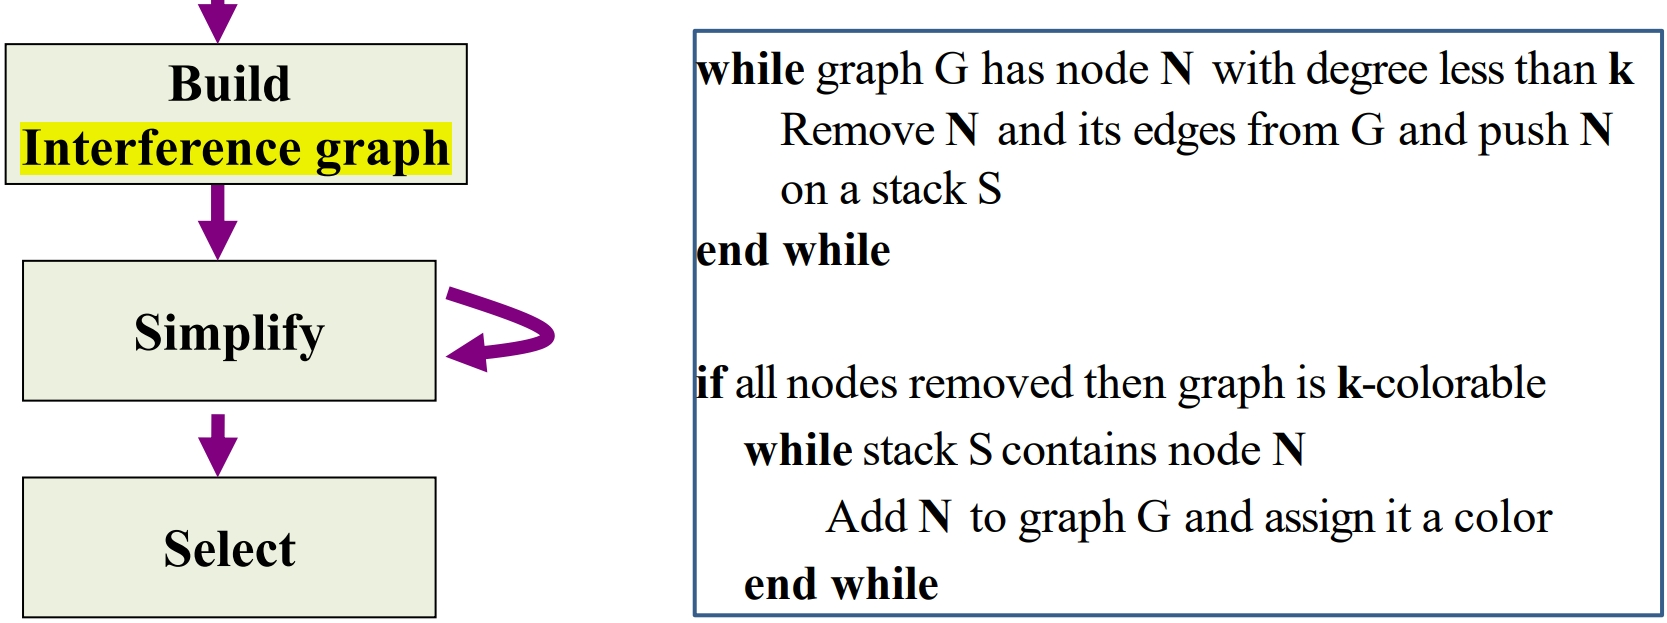
\includegraphics[width=0.8\linewidth]{figures/ra1.png}
\end{figure}

\par \noindent 上面的算法可能会失效,需要 coalescing。保守的 coalesce 对两个候选节点是否能够合并的判据(二选一):
1. (Briggs:avoid creation of high-degree $(\geq K)$ nodes)如果合并后的节点拥有小于 $K$ 个 significant 邻居;
2. (George)如果合并前,a 的每一个邻居要么是 b 的邻居,要么是 insignificant,则可以合并 ab。

\begin{figure}[H]
    \centering
    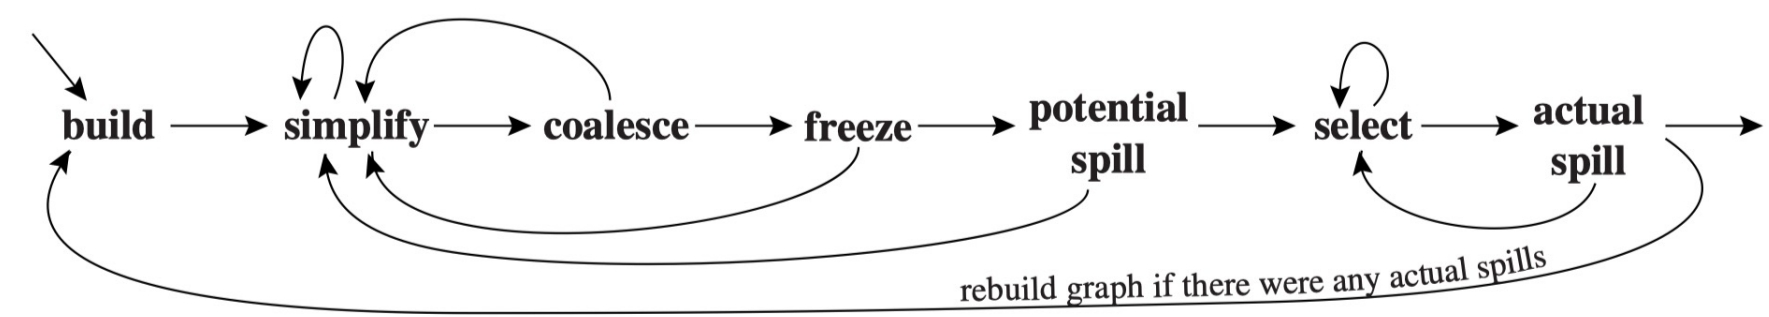
\includegraphics[width=0.8\linewidth]{figures/ra2.png}
\end{figure}

\par \noindent 1. build:构建相关图(包括虚线);
2. simplify:将图中 insignificant、non-move-related 节点移除,加入栈中;
3. coalesce:合并节点,重复 2 和 3 直到所有节点都是 significant 或者 move-related(但不能合并);
4. freeze:将低度的 move-related 节点视为 non-move-related,返回 2;
5. spill:选择高度节点进行 spill,将其移除,加入 remove 列表中,然后加入栈中(optimistic coloring);
6. select:从栈中弹出节点,将其着色,直到所有节点都被着色;
7. 如果遇到无法着色的节点,则意味着要做 actual spill,重新生成代码,生成相关图,重复。

\par \noindent Spill priority $= \frac{(\text{Use+Def Outside loop}) + 10 \times (\text{Use+Def inside loop})}{\text{Degree}}$(经验公式),
spill 这个数值最低的节点。

\par \noindent 预着色节点:不能被 simplify,不能被 spill。此时着色算法的目的是删除除了预着色节点以外的所有节点。

\par \noindent Callee-save register:Any variable that is live across several procedure calls;
Caller-save register:A local variable or compiler temporary that is not live across any procedure call。